\documentclass[12pt]{article}

\usepackage[margin=1in]{geometry}
\usepackage{amsmath}
\usepackage{amssymb}
\usepackage{physics}
\usepackage{array}
\usepackage{graphicx}
\usepackage{float}
\usepackage{tikz}
\usepackage{hyperref}
\usetikzlibrary{arrows.meta}

\title{A Systems-Oriented Introduction to Modern Retrieval}
\author{Saraansh Wadkar}
\date{}

\begin{document}

\maketitle
\tableofcontents
\newpage

\section{The Retrieval Problem}

Suppose we have a collection of documents and a user asks a question. The
system needs to find the parts of those documents that are relevant to the
query. The documents might be product descriptions, support tickets, legal
contracts, code files, research papers, or internal company notes. The
core job is simple to state: given a query, return the text that is most
likely to help.

\subsection{Raw Keyword Search}

The simplest version is keyword search. If the query is ``Toyota RAV4,''
we can look for catalog entries that contain the words ``Toyota'' and
``RAV4.'' Exact terms often matter a lot. Model names, trims, years,
drivetrain labels, engine codes, and VINs usually need literal matching.

But raw keyword search is brittle. Suppose a user asks for:

\begin{quote}
``vehicle good for off-road adventures''
\end{quote}

The best result might say ``compact SUV with all-wheel drive'' or
``pickup truck built for rough terrain.'' Those documents are relevant,
but the exact query words may not appear. A literal keyword search can
still miss them because the wording does not overlap enough.

\subsection{TF-IDF: Making Word Counts Less Naive}

One natural improvement is to score a document by counting how often the
query words appear. If the query is ``electric sedan,'' a listing that
mentions ``electric'' and ``sedan'' several times probably deserves more
attention than a listing that mentions each word once in passing. This is
the term frequency part: how often does this term appear here?

But raw counts have an obvious problem. Some words are everywhere. Words
like ``the,'' ``is,'' and ``good'' should not carry much weight. A rare
term like \texttt{RAV4}, \texttt{AWD}, ``hybrid,'' or ``hatchback'' should
matter much more because it narrows the search quickly.

That gives us the intuition behind TF-IDF. Term frequency asks how much a
term appears in this document. Inverse document frequency captures how
rare that term is across the whole collection. A good search term often
shows up in this document without showing up everywhere else.

TF-IDF is still lexical search, though. It can rank overlapping words more
carefully, but it still needs overlap. If the query says ``vehicle'' and
the document says ``SUV,'' TF-IDF does not know those ideas are related.

\subsection{BM25: A Stronger Lexical Baseline}

TF-IDF gets the basic rare-word intuition right, but practical ranking has
a few more wrinkles. After TF-IDF, the next question is not just which
words matter. We also need to decide how repeated matches should change
the score.

Repetition helps, but only up to a point. The first few mentions of a term
like ``electric'' are strong evidence that a listing is really about an
electric car. More mentions still help, but each extra mention tells us a
little less than the one before it. Repetition should have diminishing
returns. A document that mentions ``electric'' five times is probably more
relevant than one that mentions it once. A document that repeats
``electric'' 50 times is not 50 times better.

Document length causes another problem. Long documents have more chances
to contain any query term, so they can look relevant just because they
have more words. A long dealership page or family-car roundup naturally
has more opportunities to mention ``electric,'' ``SUV,'' or ``AWD'' than a
short listing does. But that does not mean it is the better match. A short
listing that says ``electric sedan with long range'' should probably rank
above a long overview that mentions ``electric sedan'' once among 20
different vehicles.

BM25 is a practical way to rank lexical matches by combining three
intuitions: some terms matter more than others, repeated matches should
help with diminishing returns, and long documents need a correction so
they do not win by default. It is still based on words, but it is a strong
baseline for exact terms: model names, trims, VINs, drivetrain labels,
engine types, and rare phrases. When exact wording matters, BM25 is often
a very good fit.

\subsection{Where Lexical Search Still Breaks}

TF-IDF and BM25 are useful, but they still mostly match words rather than
meaning. They struggle with synonyms, paraphrases, and vague
natural-language queries. ``Car'' and ``vehicle'' may refer to the same
thing. ``Good for rough terrain'' and ``built for off-road use'' are close
in meaning without being the same sentence. A document that says
``compact SUV with all-wheel drive'' may still be a good answer to a query
about ``off-road adventures,'' even if the words barely line up.

This is where semantic search helps. Instead of comparing text only by
word overlap, it maps both the documents and the query into vectors. Those
vectors are arranged so that related meanings tend to land near each
other. At that point the question is no longer ``which documents contain
these words?'' but ``which stored meanings are closest to this query?''

\section{Semantic Search}

Semantic search works by turning both queries and documents into vectors
that preserve meaning geometrically. If related ideas land near each
other, then retrieval can work from semantic closeness instead of relying
only on overlapping words.

\subsection{What Is a Vector?}

In the context of embeddings and vector databases, a vector is an
$n$-dimensional ordered list of numbers:
\[
\mathbf{v} = [v_1, v_2, \dots, v_n].
\]
In practice, each coordinate is usually stored as a signed 32-bit
floating-point value, so a single vector is often represented as an
$n$-dimensional array of 4-byte floats.

An embedding vector is useful because it encodes semantic meaning into
geometry. Rather than storing meaning in words or symbols directly, the
model maps text, images, or other data into a point in a high-dimensional
space. Items with similar meaning are placed closer together, while items
with different meanings are placed farther apart.

For example, two sentences about databases may produce vectors that point
in similar directions, even if they do not share the exact same words.
This is what makes vector search possible: we compare the geometry of
embeddings instead of relying only on exact keyword matches.

\subsection{How Embeddings Are Created}

The key question is how a piece of text becomes a useful vector at all.
Modern embedding models are more complicated than the simplified story I
am giving here. There is a lot going on under the hood, and there is a
substantial literature on how these models tokenize text, build internal
representations, and produce final embeddings. For our purposes, though,
we can treat the model as a black box: it takes in text and returns an
$n$-dimensional vector that captures enough semantic information to make
similarity comparisons useful. In practice, texts with related meanings
tend to end up near each other in that space, even when the wording is
different.

An embedding model first breaks text into smaller units called tokens.
Those tokens are then processed by a neural network that has been trained
on very large amounts of data. During training, the model learns internal
patterns about which words, phrases, and concepts tend to appear in
similar contexts.

By the time the model is used for embeddings, it has learned to map text
into a high-dimensional latent space. Each coordinate in the output vector
is a learned scalar value. The model was not told ahead of time that
dimension 17 should mean ``animal'' or that dimension 243 should mean
``database.'' Those labels are not built in. Still, the numbers are not
random. Training pushes the model to arrange them so that useful patterns
show up in the geometry of the space.

This is why embeddings are deeper than just lists of floats. A coordinate
can carry semantic signal, but that signal is usually not cleanly labeled
or easy to isolate. One direction in the space might roughly line up with
something like ``more technical,'' ``more emotional,'' ``more physical
object,'' or ``more finance-related.'' That does not mean there is a neat
technicalness dimension that we can read directly. It means the model has
learned directions and combinations of coordinates that tend to matter for
the data it saw during training.

The sign and size of a scalar matter too, but only inside the learned
space. A positive value points one way along that coordinate or direction.
A negative value points the opposite way. A larger absolute value means
that coordinate contributes more strongly to the vector's position.
However, a single coordinate rarely explains the meaning by itself. The
meaning is usually spread across many dimensions, and the full vector
matters as a whole. Two embeddings end up close because many of these
learned signals line up together. That is why cosine similarity compares
the direction of the whole vector rather than reading one number at a
time.

For a deeper intuition, 3Blue1Brown has a short video on how directions or
dimensions in these spaces can pick up semantic meaning in
\href{https://youtube.com/shorts/FJtFZwbvkI4?si=rtebhzbhDrnXiyIL}{this
3Blue1Brown video}.

For example, suppose we embed the sentence ``the cat sat on the mat.'' The
model first tokenizes it into pieces such as ``the'', ``cat'', ``sat'',
``on'', ``the'', and ``mat''. Those tokens are passed through many layers
of the network, which combine all of those learned signals into a single
output vector such as
\[
\mathbf{e}_{\text{cat}} = [0.12, -0.44, 0.91, \dots, 0.08].
\]
The exact numbers are not human-interpretable on their own. What matters
is that another sentence like ``a kitten is resting on a rug'' will likely
produce a vector in a nearby region of the space, because the model has
learned that ``cat'' and ``kitten'' are related concepts and that both
sentences describe similar situations.

As a result, text with similar meaning tends to produce vectors that end
up near each other, even when the wording changes. The embedding works
because the model has compressed many layers of statistical and semantic
structure into a numerical representation that preserves useful similarity
relationships.

\subsection{Semantic Search Example}

Suppose you are shopping for a car and want something good for
off-road adventures. You have a small catalog of cars, each with a short
description. At first this sounds like a simple search problem, but there
is an immediate issue: none of the descriptions may literally contain the
phrase ``off-road adventures.'' A plain keyword search or \texttt{Ctrl+F}
style lookup would therefore miss relevant cars even if some of them are
actually a good fit.

Here is the dataset:

\begin{enumerate}
    \item ``Tesla Model 3 is an electric sedan designed for daily commuting with great efficiency''
    \item ``Ford F-150 is a powerful pickup truck built for hauling and towing heavy loads''
    \item ``Toyota RAV4 is a compact SUV with good fuel economy and family-friendly features''
    \item ``Porsche 911 is a high-performance sports car built for speed and handling''
    \item ``Honda Civic is a reliable compact car ideal for commuting''
    \item ``Chevy Bolt is an affordable electric hatchback for city driving''
\end{enumerate}

The Ford F-150 and Toyota RAV4 might both be relevant to an
``off-road adventures'' style query, but neither description uses those
exact words. So how do we search by meaning instead of by exact text?

The key idea is to embed each description into a vector. Conceptually,
each record might look like:

\begin{verbatim}
{
  car_name: "Tesla Model 3",
  description: "Electric sedan for efficient daily commuting",
  vector: [...] 
}
\end{verbatim}

The important point is that the \texttt{vector} is produced from the
\texttt{description}. Once all the descriptions are embedded, we do the
same thing to the user's query:

\begin{quote}
``vehicle good for off-road adventures''
\end{quote}

In this situation, the Toyota RAV4 and Ford F-150 might rank higher than
the Tesla Model 3 or Honda Civic, even though none of the descriptions
contain the exact phrase ``off-road adventures.'' The system works because
the embedding model has placed related meanings in nearby parts of the
vector space. This is the core promise of semantic search: retrieve by
meaning, not just by literal keyword overlap.

\begin{figure}[h]
\centering
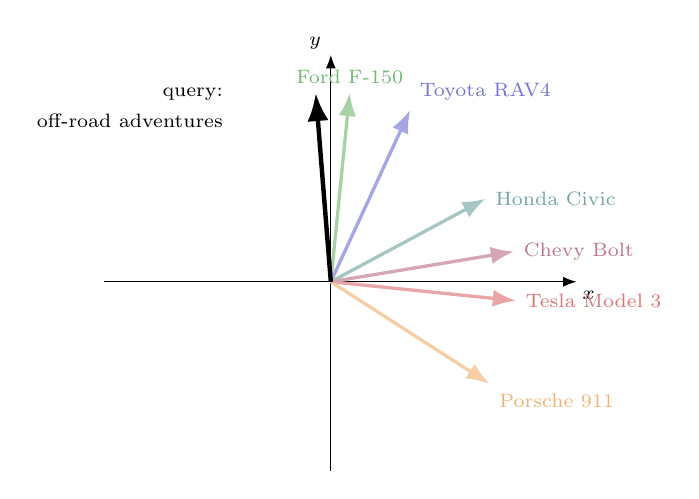
\begin{tikzpicture}[scale=2.4, >=Latex]
    \draw[->, thin] (-1.2,0) -- (1.3,0);
    \draw[->, thin] (0,-1.0) -- (0,1.2);
    \node[below right] at (1.28,0) {\scriptsize $x$};
    \node[above left] at (0,1.18) {\scriptsize $y$};

    \draw[->, very thick, red!75!black!35] (0,0) -- (0.98,-0.10);
    \node[red!75!black!55, right] at (0.98,-0.10) {\scriptsize Tesla Model 3};

    \draw[->, very thick, blue!70!black!35] (0,0) -- (0.42,0.91);
    \node[blue!70!black!55, above right] at (0.42,0.91) {\scriptsize Toyota RAV4};

    \draw[->, very thick, green!50!black!35] (0,0) -- (0.10,1.00);
    \node[green!50!black!55, above] at (0.10,1.00) {\scriptsize Ford F-150};

    \draw[->, very thick, orange!90!black!35] (0,0) -- (0.84,-0.54);
    \node[orange!90!black!55, below right] at (0.84,-0.54) {\scriptsize Porsche 911};

    \draw[->, very thick, teal!70!black!35] (0,0) -- (0.82,0.44);
    \node[teal!70!black!55, right] at (0.82,0.44) {\scriptsize Honda Civic};

    \draw[->, very thick, purple!70!black!35] (0,0) -- (0.97,0.16);
    \node[purple!70!black!55, right] at (0.97,0.16) {\scriptsize Chevy Bolt};

    \draw[->, ultra thick, black] (0,0) -- (-0.08,1.00);
    \node[black, left, align=right] at (-0.52,0.92) {\scriptsize query:\\[-1pt]\scriptsize off-road adventures};
\end{tikzpicture}
\caption{A 2D picture of semantic similarity. Real embeddings are
high-dimensional, but the same directional intuition applies.}
\end{figure}

This picture is only 2D, while real embeddings live in much higher
dimensions, but it captures the basic idea. Cars that are close together
have similar descriptions. The Tesla Model 3, Honda Civic, and Chevy Bolt
cluster in a more commuting- and city-driving-oriented direction. The
Toyota RAV4 and Ford F-150 sit much closer to each other because their
descriptions both emphasize utility. The query vector for
``off-road adventures'' also points in that same general direction, which
is why those vehicles would be better matches.

At that point, the natural question becomes: how can we mathematically
find which vectors are most similar?

\subsubsection{Cosine Similarity}

Once we have a query vector and a set of car vectors, we need a
mathematical way to ask: which vectors point in the most similar
direction? One of the most common answers is cosine similarity. Given
vectors $\mathbf{u}$ and $\mathbf{v}$, their cosine similarity is
\[
\cos(\theta) =
\frac{\mathbf{u} \cdot \mathbf{v}}{\norm{\mathbf{u}} \norm{\mathbf{v}}}.
\]

Intuitively, this is about angle. If two vectors point in almost the same
direction, then the angle between them is close to $0^\circ$, and
$\cos(0^\circ) = 1$. That means the vectors are highly similar. If the
angle is around $90^\circ$, then $\cos(90^\circ) = 0$, which means they
are effectively unrelated. If they point in opposite directions, the angle
approaches $180^\circ$ and the cosine becomes negative.

We can make that concrete by isolating the query vector and comparing it
against a few individual cars:

\begin{figure}[h]
\centering
\begin{minipage}[t]{0.31\textwidth}
\centering
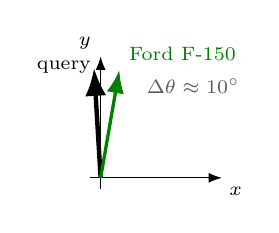
\begin{tikzpicture}[scale=1.4, >=Latex]
    \draw[->, thin] (-0.1,0) -- (1.1,0);
    \draw[->, thin] (0,-0.1) -- (0,1.1);
    \node[below right] at (1.08,0) {\scriptsize $x$};
    \node[above left] at (0,1.08) {\scriptsize $y$};
    \draw[->, ultra thick, black] (0,0) -- (-0.06,1.0);
    \draw[->, very thick, green!50!black] (0,0) -- (0.17,0.98);
    \node[gray!70!black] at (0.84,0.83) {\scriptsize $\Delta \theta \approx 10^\circ$};
    \node[black, left] at (0,1.0) {\scriptsize query};
    \node[green!50!black, above right] at (0.17,0.98) {\scriptsize Ford F-150};
\end{tikzpicture}

\vspace{0.2em}
\scriptsize High similarity: $\cos(10^\circ) \approx 0.98$. The query and
Ford point in almost the same direction, so this is a strong semantic
match.
\end{minipage}
\hfill
\begin{minipage}[t]{0.31\textwidth}
\centering
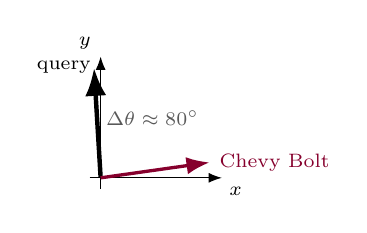
\begin{tikzpicture}[scale=1.4, >=Latex]
    \draw[->, thin] (-0.1,0) -- (1.1,0);
    \draw[->, thin] (0,-0.1) -- (0,1.1);
    \node[below right] at (1.08,0) {\scriptsize $x$};
    \node[above left] at (0,1.08) {\scriptsize $y$};
    \draw[->, ultra thick, black] (0,0) -- (-0.06,1.0);
    \draw[->, very thick, purple!70!black] (0,0) -- (0.99,0.14);
    \node[gray!70!black] at (0.47,0.54) {\scriptsize $\Delta \theta \approx 80^\circ$};
    \node[black, left] at (0,1.0) {\scriptsize query};
    \node[purple!70!black, right] at (0.99,0.14) {\scriptsize Chevy Bolt};
\end{tikzpicture}

\vspace{0.2em}
\scriptsize Weak similarity: $\cos(80^\circ) \approx 0.17$. Both are
vehicles, but the meanings are mostly different, so this is close to
noise.
\end{minipage}
\hfill
\begin{minipage}[t]{0.31\textwidth}
\centering
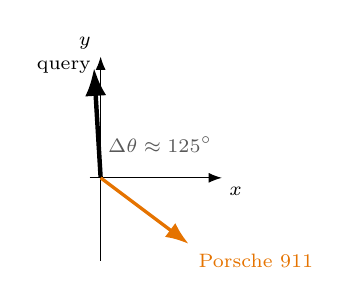
\begin{tikzpicture}[scale=1.4, >=Latex]
    \draw[->, thin] (-0.1,0) -- (1.1,0);
    \draw[->, thin] (0,-0.75) -- (0,1.1);
    \node[below right] at (1.08,0) {\scriptsize $x$};
    \node[above left] at (0,1.08) {\scriptsize $y$};
    \draw[->, ultra thick, black] (0,0) -- (-0.06,1.0);
    \draw[->, very thick, orange!90!black] (0,0) -- (0.80,-0.60);
    \node[gray!70!black] at (0.54,0.30) {\scriptsize $\Delta \theta \approx 125^\circ$};
    \node[black, left] at (0,1.0) {\scriptsize query};
    \node[orange!90!black, below right] at (0.80,-0.60) {\scriptsize Porsche 911};
\end{tikzpicture}

\vspace{0.2em}
\scriptsize Negative similarity: $\cos(125^\circ) \approx -0.57$. This
vector points in a very different direction, so it is a poor match for the
query.
\end{minipage}
\caption{Cosine similarity compares the angle between the query vector and
each car vector. Small angles mean high similarity; large angles mean weak
or even negative similarity.}
\end{figure}

In the car-shopping example, we would compute the cosine similarity
between the query vector and each car description vector, then sort the
results from highest to lowest score. If the query vector points in a
similar direction to the Toyota RAV4 vector, that suggests their meanings
are related even though the query says ``off-road adventures'' and the
description says ``compact SUV.'' This is exactly why cosine similarity is
useful: it lets us retrieve semantically related results without needing
the same literal words to appear in both strings.

In practice, cosine similarity scores are often interpreted as rough
relevance signals. A score around $0.9$ usually indicates a very strong
match. Around $0.7$ is often still meaningfully related, but less precise.
Around $0.4$ is more borderline: there may be some overlap in topic or
context, but the match is weak. Around $0.2$ is often close to noise.
These are heuristics rather than hard rules, since the exact thresholds
depend on the embedding model and the dataset.

The same idea is not limited to language. Vector representations can also
capture similarity for numbers and other structured features. If two data
points have similar numerical patterns, their vectors may still end up
close together, allowing the database to retrieve values that are
numerically or structurally related rather than only textually related.

\subsection{Piecing it together}

At this point, we have two ingredients: a way to turn data into vectors
and a way to compare those vectors. The natural next question is what
kind of structure would let us use those ingredients in a real system.
Having individual vectors is not enough on its own. We need some
organized way to store them alongside the data they came from so that a
query can return something useful to a user rather than just a list of
floating-point numbers.

The simplest useful structure is a collection of records where each
record contains the original content, its embedding vector, and whatever
extra metadata we may want to keep around. Conceptually, a single entry
might look like this:

\begin{verbatim}
{
  id: 42,
  content: "Toyota RAV4 is a compact SUV with good fuel economy",
  embedding: [...],
  metadata: {
    brand: "Toyota",
    type: "SUV"
  }
}
\end{verbatim}

Once the data is arranged this way, the workflow becomes much clearer. We
embed each document, sentence, image caption, or product description
ahead of time and store the resulting vector with the original record.
Later, when a user submits a query, we embed the query into its own
vector, compare it against the stored vectors, and return the records
whose embeddings are closest. In other words, the useful structure is not
just ``a pile of vectors,'' but a searchable collection of data where
each vector remains tied to the object it represents.

This is the basic idea behind semantic retrieval. Embeddings let us search
by meaning, not just by literal wording. That is powerful on its own, but
real systems often combine semantic retrieval with lexical retrieval
rather than choosing only one.

\section{Hybrid Search}

Once we understand lexical retrieval and semantic retrieval separately,
the practical question becomes: how do we combine them? BM25 and semantic
retrieval are not competing answers to the same problem. They are good at
different things. BM25 is strong when exact wording matters. Vector
retrieval is strong when meaning matters even though the words change.

\subsection{Why Combine Lexical and Semantic Retrieval?}

Neither retriever is universally better. If the query is ``Toyota RAV4
AWD,'' exact lexical matching should matter a lot. A result that contains
those exact words is probably important. But if the query is ``vehicle
good for off-road adventures,'' we still want to surface things like a
Toyota RAV4, Ford F-150, or Subaru Outback even if the wording in the
documents is different.

That is why hybrid retrieval is useful. We can run a lexical retriever
such as BM25 and a semantic retriever based on embeddings, then combine
their candidate lists. Score blending is one option, but raw lexical
scores and vector similarity scores often live on different scales. In
practice, simple rank-based fusion methods are often easier to reason
about.

\subsection{Reciprocal Rank Fusion (RRF)}

One common rank-based method is reciprocal rank fusion, usually shortened
to RRF. The idea is simple: if a document appears near the top of several
ranked lists, it should get a higher combined score.

\[
\mathrm{RRF}(d) = \sum_i \frac{1}{k + \mathrm{rank}_i(d)}
\]

Here, $d$ is a document or chunk. Each retriever contributes one term to
the sum. $\mathrm{rank}_i(d)$ is where that item appeared in retriever
$i$'s ranked list. Smaller ranks contribute more, since being ranked $1$
is better than being ranked $10$. The constant $k$ smooths the effect so
that one top rank does not dominate too aggressively.

We can make that concrete with a small car-search example. Let us set
$k = 10$ so the arithmetic stays easy to inspect. Suppose the user query
is:

\begin{quote}
``Toyota RAV4 AWD for off-road adventures''
\end{quote}

Now suppose BM25 and vector search each return a ranked list:

\begin{center}
\begin{tabular}{|c|c|c|c|c|}
\hline
vehicle & BM25 rank & vector rank & RRF score & RRF rank \\
\hline
Toyota RAV4 & 1 & 4 & $\frac{1}{11}+\frac{1}{14}\approx 0.162$ & 2 \\
Ford F-150 & 2 & 1 & $\frac{1}{12}+\frac{1}{11}\approx 0.174$ & 1 \\
Subaru Outback & 5 & 2 & $\frac{1}{15}+\frac{1}{12}\approx 0.150$ & 3 \\
\hline
\end{tabular}
\end{center}

BM25 strongly favors the Toyota RAV4 because the query contains those
exact words. Vector search strongly favors the Ford F-150 because it looks
semantically close to the ``off-road adventures'' part of the query.
Ford wins the fused ranking because it is near the top of both lists.
Toyota stays strong because rank 1 in BM25 still matters a lot. Subaru is
rewarded for appearing near the top of both lists too, but in this example
its combined score is still lower than Ford's and Toyota's. That is the
appeal of RRF: it rewards agreement across retrievers without requiring
their raw scores to live on the same scale.

\subsection{From Fusion to Reranking}

Hybrid retrieval gives us a better candidate set, but it still does not
guarantee the final ordering is perfect. A common next step is to fuse the
lexical and vector candidates first, then pass the merged list into a
reranker that can compare the query and candidates more carefully.

At that point, we have a clear picture of the retrieval behavior we want:
lexical search, semantic search, fusion, and then reranking. The next
systems question is how to store that data and search it efficiently at
scale.

\section{From B-Trees to Vector Indexes}

Before we talk about vector databases, it helps to look at how ordinary
databases make search fast in the first place. The next couple of
subsections cover database ideas that some readers may already know, so
they can be skimmed if indexes and B-trees are familiar. They are still
worth setting up because vector databases are built around the same basic
split between storing data and searching it quickly.

\subsection{Why Databases Need Indexes}

The simplest way to search a table is to look through it row by row. If a
database sees a query like this:

\begin{verbatim}
SELECT * FROM users WHERE id = 42;
\end{verbatim}

it could check the first row, then the second row, then the third row, and
keep going until it finds the matching record. This is a linear scan,
often called a full table scan when the database has to consider the
whole table.

That approach is simple and correct. For 100 rows, it may be fine. For
100 million rows, doing that on every request is a problem. The amount of
work grows with the size of the table, even if the query only needs one
record.

Indexes exist to avoid that kind of scan. A database index is a separate
data structure built from selected column values and pointers back to the
underlying rows. It does not replace the table. It gives the database a
faster path to the rows that matter.

A scalar index is an index over one ordinary value per row, such as an
integer ID, timestamp, username, price, or category. These are values that
can be compared directly. Scalar indexes help with exact matches, ranges,
and sorted order. Without an index, the database may have to scan each row
and check whether \texttt{id = 42}. With an index on \texttt{id}, it can
search the index first, find the row location, and then fetch the matching
record.

\subsection{B-Trees: A Common Scalar Index}

A B-tree is one common way to implement a scalar index. At a high level,
a B-tree keeps keys in sorted order and stores them in a balanced tree.
That balance matters because it keeps the tree from becoming a long
lopsided chain. Instead of checking rows one by one, the database can
follow the tree downward and quickly narrow the search to a smaller part
of the data.

This is a good fit for the kinds of questions relational databases answer
all the time:

\begin{verbatim}
SELECT * FROM users WHERE id = 42;
SELECT * FROM orders WHERE created_at > '2026-01-01';
\end{verbatim}

In both cases, the database is working with values that have a natural
sorted order. An ID can be ordered numerically. A timestamp can be ordered
chronologically. Once the keys are sorted, the database can ask a simple
question: where would this value fall in that ordering?

\begin{figure}[H]
\centering
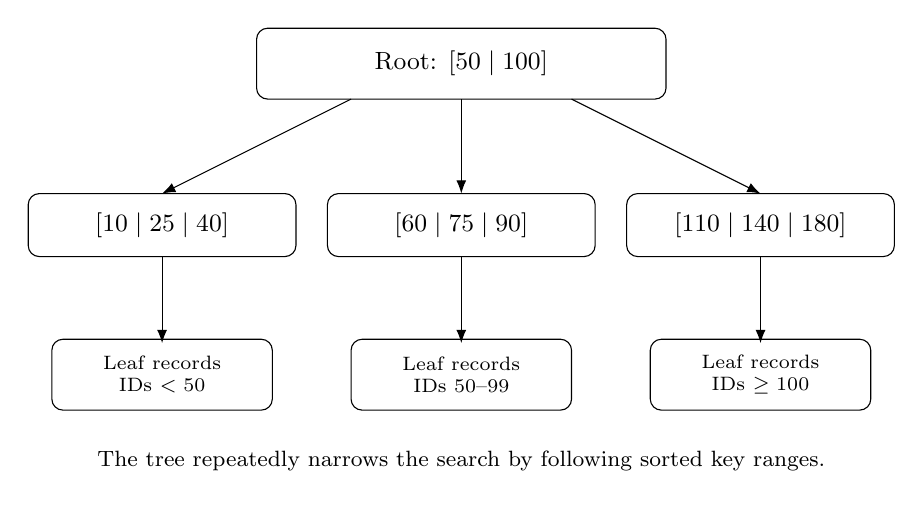
\begin{tikzpicture}[>=Latex, every node/.style={font=\small}]
    \draw[rounded corners] (3.4,4.5) rectangle (8.6,5.4);
    \node at (6.0,4.95) {Root: $[50 \mid 100]$};

    \draw[->] (4.6,4.5) -- (2.2,3.3);
    \draw[->] (6.0,4.5) -- (6.0,3.3);
    \draw[->] (7.4,4.5) -- (9.8,3.3);

    \draw[rounded corners] (0.5,2.5) rectangle (3.9,3.3);
    \node at (2.2,2.9) {$[10 \mid 25 \mid 40]$};

    \draw[rounded corners] (4.3,2.5) rectangle (7.7,3.3);
    \node at (6.0,2.9) {$[60 \mid 75 \mid 90]$};

    \draw[rounded corners] (8.1,2.5) rectangle (11.5,3.3);
    \node at (9.8,2.9) {$[110 \mid 140 \mid 180]$};

    \draw[->] (2.2,2.5) -- (2.2,1.4);
    \draw[->] (6.0,2.5) -- (6.0,1.4);
    \draw[->] (9.8,2.5) -- (9.8,1.4);

    \draw[rounded corners] (0.8,0.55) rectangle (3.6,1.45);
    \node[align=center, font=\scriptsize] at (2.2,1.0) {Leaf records\\ IDs $< 50$};

    \draw[rounded corners] (4.6,0.55) rectangle (7.4,1.45);
    \node[align=center, font=\scriptsize] at (6.0,1.0) {Leaf records\\ IDs $50$--$99$};

    \draw[rounded corners] (8.4,0.55) rectangle (11.2,1.45);
    \node[align=center, font=\scriptsize] at (9.8,1.0) {Leaf records\\ IDs $\ge 100$};

    \node[align=center] at (6.0,-0.1) {\footnotesize The tree repeatedly narrows the search by following sorted key ranges.};
\end{tikzpicture}
\caption{A simple B-tree-style search intuition. The database does not
scan every row. It follows ordered key ranges until it reaches the small
part of the table that could contain the answer.}
\end{figure}

That is why B-trees are so useful. They are great when the thing being
indexed has a clean one-dimensional ordering. Equality queries, range
queries, and ordered scans all fit that pattern nicely.

\subsection{Why This Breaks for Embeddings}

Scalar indexes work because scalar values can be sorted in one clean
order. Embeddings do not fit that pattern nearly as well. An embedding is
not one number that can be dropped into a sorted list. It is a long vector
such as
\[
[0.12, -0.44, 0.91, \dots, 0.08].
\]

Once the data looks like that, the query changes too. We are no longer
asking:

\begin{verbatim}
WHERE id = 42
WHERE created_at > ...
\end{verbatim}

Now we are asking something much stranger:

\begin{quote}
Which stored vectors are closest to this new vector under cosine
similarity or distance?
\end{quote}

That is a different kind of problem. A B-tree helps when the question is
``where does this value belong in sorted order?'' Vector search asks
``which points are nearby in space?'' There is no single sorted order of
high-dimensional vectors that preserves semantic closeness in the way a
sorted list of IDs preserves numeric order. Two vectors can be close in
meaning even if many of their individual coordinates differ in messy ways.
The whole geometry matters, not one field. That is why vector search needs
a different kind of index.

\begin{figure}[h]
\centering
\begin{minipage}[t]{0.46\textwidth}
\centering
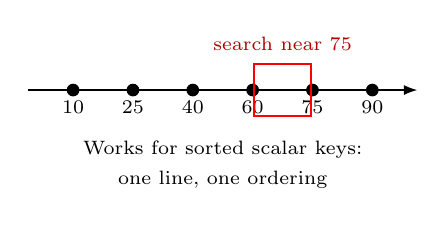
\begin{tikzpicture}[>=Latex, scale=0.95]
    \draw[->] (0,0) -- (5.2,0);
    \foreach \x/\label in {0.6/10,1.4/25,2.2/40,3.0/60,3.8/75,4.6/90}
    {
        \filldraw[black] (\x,0) circle (2.2pt);
        \node[below] at (\x,-0.02) {\scriptsize \label};
    }
    \draw[thick, red] (3.02,-0.35) rectangle (3.78,0.35);
    \node[above, red!70!black] at (3.4,0.4) {\scriptsize search near 75};
    \node[align=center] at (2.6,-1.0) {\scriptsize Works for sorted scalar keys:\\[-1pt]\scriptsize one line, one ordering};
\end{tikzpicture}
\end{minipage}
\hfill
\begin{minipage}[t]{0.46\textwidth}
\centering
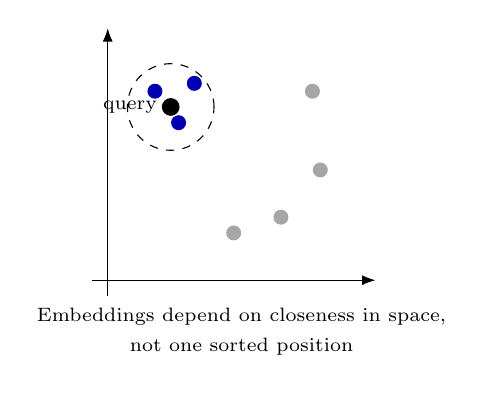
\begin{tikzpicture}[>=Latex, scale=1.0]
    \draw[->, thin] (-0.2,0) -- (3.4,0);
    \draw[->, thin] (0,-0.2) -- (0,3.2);
    \filldraw[blue!70!black] (0.6,2.4) circle (2.5pt);
    \filldraw[blue!70!black] (0.9,2.0) circle (2.5pt);
    \filldraw[blue!70!black] (1.1,2.5) circle (2.5pt);
    \filldraw[gray!70] (2.6,2.4) circle (2.5pt);
    \filldraw[gray!70] (2.7,1.4) circle (2.5pt);
    \filldraw[gray!70] (2.2,0.8) circle (2.5pt);
    \filldraw[gray!70] (1.6,0.6) circle (2.5pt);
    \filldraw[black] (0.8,2.2) circle (3pt);
    \draw[dashed] (0.8,2.2) circle (0.55);
    \node[left] at (0.75,2.2) {\scriptsize query};
    \node[align=center] at (1.7,-0.65) {\scriptsize Embeddings depend on closeness in space,\\[-1pt]\scriptsize not one sorted position};
\end{tikzpicture}
\end{minipage}
\caption{Why sorted order stops helping. On the left, a database can use a
single ordered key to zoom in on the answer. On the right, semantic search
depends on geometric closeness in a space of vectors.}
\end{figure}

This is the point where retrieval enters the story.

\subsection{What Retrieval Means Here}

In the embedding setting, retrieval means this: given a query vector,
return the stored records whose vectors are nearest to it under some
similarity measure. Those results are called the query's nearest
neighbors.

That phrase can sound more mysterious than it really is. A nearest
neighbor is just one of the stored vectors that sits closest to the query
point in the embedding space. If we use cosine similarity, we are asking
which vectors point in the most similar direction. If we use Euclidean
distance, we are asking which vectors lie physically closest in that
space.

\subsection{Exact Search First}

The simplest way to do this is also the most brute-force. We embed the
query, compare it against every stored vector, compute a score for each
one, sort the results, and return the top $k$. That is exact
nearest-neighbor search.

It is easy to understand, and it gives the true top results for the
chosen similarity measure. For a small dataset, that may be perfectly
fine. But if the database holds millions of vectors, doing that much work
for every query starts to hurt. The system may have to score the query
against every row, even though only a handful of rows will make the final
cut.

\subsection{Approximate Search and HNSW}

That scaling problem is why many vector databases use approximate nearest
neighbor search, usually shortened to ANN. The word ``approximate'' is
important. ANN methods do not promise the mathematically exact best answer
every time. Instead, they try to return very good neighbors much faster
than a full scan.

One of the most common ANN structures is HNSW, which stands for
Hierarchical Navigable Small World. The name is a mouthful, but the basic
idea is manageable. HNSW stores vectors in a graph. Each vector is linked
to other vectors that are nearby. Search starts from a coarse upper layer,
moves toward a promising region, and then drops into denser lower layers
for a more local search. So instead of comparing the query with every
stored vector, the system walks through the graph toward better matches.

\begin{figure}[h]
\centering
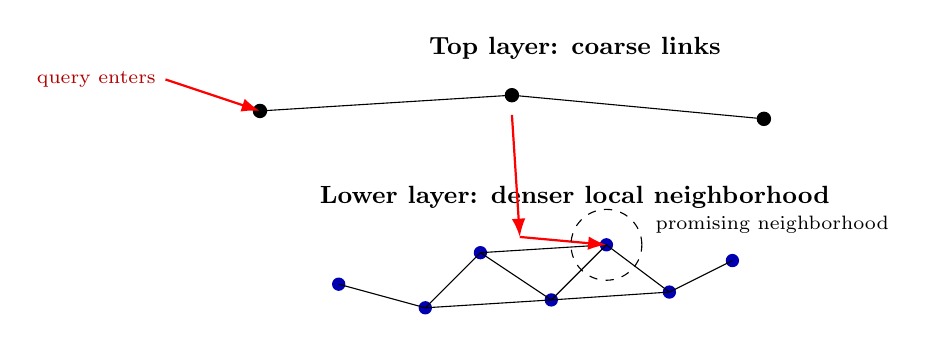
\begin{tikzpicture}[>=Latex, every node/.style={font=\small}]
    \node at (6.0,4.4) {\textbf{Top layer: coarse links}};
    \filldraw[black] (2.0,3.6) circle (2.4pt);
    \filldraw[black] (5.2,3.8) circle (2.4pt);
    \filldraw[black] (8.4,3.5) circle (2.4pt);
    \draw (2.0,3.6) -- (5.2,3.8) -- (8.4,3.5);
    \draw[->, thick, red] (0.8,4.0) -- (2.0,3.6);
    \node[left, red!70!black] at (0.8,4.0) {\scriptsize query enters};

    \node at (6.0,2.5) {\textbf{Lower layer: denser local neighborhood}};
    \foreach \x/\y in {3.0/1.4,4.1/1.1,4.8/1.8,5.7/1.2,6.4/1.9,7.2/1.3,8.0/1.7}
        \filldraw[blue!70!black] (\x,\y) circle (2.2pt);
    \draw (3.0,1.4) -- (4.1,1.1) -- (4.8,1.8) -- (5.7,1.2) -- (6.4,1.9) -- (7.2,1.3) -- (8.0,1.7);
    \draw (4.1,1.1) -- (5.7,1.2);
    \draw (4.8,1.8) -- (6.4,1.9);
    \draw (5.7,1.2) -- (7.2,1.3);
    \draw[->, thick, red] (5.2,3.55) -- (5.3,2.0);
    \draw[->, thick, red] (5.3,2.0) -- (6.4,1.9);
    \draw[dashed] (6.4,1.9) circle (0.45);
    \node[right] at (6.9,2.15) {\scriptsize promising neighborhood};
\end{tikzpicture}
\caption{HNSW search intuition. The search starts with coarse navigation,
then moves into a denser local neighborhood instead of scanning every
vector in the database.}
\end{figure}

HNSW is not the only option. Another common ANN structure is IVFFlat,
which groups vectors into coarse clusters first and then searches within
the most relevant ones. Instead of walking a graph, IVFFlat asks a
coarser question first: which regions of the vector space are worth
looking inside?

\begin{figure}[h]
\centering
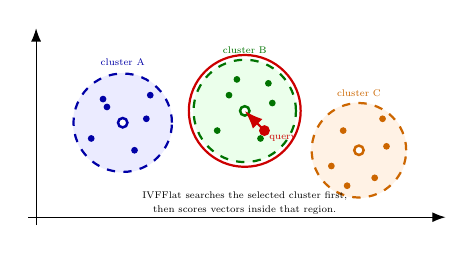
\begin{tikzpicture}[>=Latex, scale=0.50, transform shape, every node/.style={font=\small}]
    \draw[->, thin] (-0.2,0) -- (10.4,0);
    \draw[->, thin] (0,-0.2) -- (0,4.8);

    \filldraw[blue!8] (2.2,2.4) circle (1.25);
    \draw[blue!65!black, dashed, thick] (2.2,2.4) circle (1.25);
    \node[blue!65!black] at (2.2,3.95) {\scriptsize cluster A};
    \filldraw[fill=white, draw=blue!65!black, line width=0.9pt] (2.2,2.4) circle (3.4pt);
    \foreach \x/\y in {1.4/2.0,1.8/2.8,2.5/1.7,2.8/2.5,1.7/3.0,2.9/3.1}
        \filldraw[blue!65!black] (\x,\y) circle (2pt);

    \filldraw[green!8] (5.3,2.7) circle (1.3);
    \draw[green!45!black, dashed, thick] (5.3,2.7) circle (1.3);
    \node[green!45!black] at (5.3,4.25) {\scriptsize cluster B};
    \filldraw[fill=white, draw=green!45!black, line width=0.9pt] (5.3,2.7) circle (3.4pt);
    \foreach \x/\y in {4.6/2.2,4.9/3.1,5.7/2.0,6.0/2.9,5.1/3.5,5.9/3.4}
        \filldraw[green!45!black] (\x,\y) circle (2pt);

    \filldraw[orange!10] (8.2,1.7) circle (1.2);
    \draw[orange!80!black, dashed, thick] (8.2,1.7) circle (1.2);
    \node[orange!80!black] at (8.2,3.15) {\scriptsize cluster C};
    \filldraw[fill=white, draw=orange!80!black, line width=0.9pt] (8.2,1.7) circle (3.4pt);
    \foreach \x/\y in {7.5/1.3,7.8/2.2,8.6/1.0,8.9/1.8,7.9/0.8,8.8/2.5}
        \filldraw[orange!80!black] (\x,\y) circle (2pt);

    \filldraw[red!80!black] (5.8,2.2) circle (3.5pt);
    \node[red!80!black, below right] at (5.8,2.2) {\scriptsize query};
    \draw[->, thick, red!80!black] (5.8,2.2) -- (5.3,2.7);
    \draw[red!80!black, thick] (5.3,2.7) circle (1.42);
    \node[align=center] at (5.3,0.35) {\scriptsize IVFFlat searches the selected cluster first,\\[-1pt]\scriptsize then scores vectors inside that region.};
\end{tikzpicture}
\caption{IVFFlat search intuition. The dashed circles are coarse regions,
the larger filled dots are centroid vectors, and the smaller dots are
stored vectors assigned to each centroid.}
\end{figure}

HNSW is still a good main example because it shows the key idea clearly:
vector search usually depends on a special index designed for geometric
similarity, not an ordinary sorted tree.

\subsection{So What Does a Vector Database Store?}

At this point, it helps to separate storage from indexing. A vector
database still stores recognizable records. Each one usually includes the
original content, an ID, the embedding, and whatever metadata the
application needs.

\begin{verbatim}
{
  id: 42,
  content: "Toyota RAV4 is a compact SUV with good fuel economy",
  embedding: [...],
  metadata: {
    brand: "Toyota",
    type: "SUV",
    created_at: "2026-05-25"
  }
}
\end{verbatim}

Some of those fields may still use ordinary database indexes. For
example, filtering by tenant, brand, timestamp, or category may rely on
traditional indexes, often B-trees. That part of the system looks a lot
like a normal database.

The difference is that the embeddings usually get an additional vector
index built over them. That index is a separate data structure that points
back to the stored records. In an HNSW-style index, that structure looks
like a graph: each vector has links to nearby vectors, and the search
walks through those links toward better matches.

In an IVFFlat-style index, the structure looks more like a set of buckets.
The database stores a small set of centroid vectors, like the larger
center dots in the IVFFlat figure above. Each centroid represents a coarse
region of the vector space. Behind each centroid is an inverted list of
row IDs or vector IDs assigned to that region:

\begin{verbatim}
centroid_1 -> [row_id 7, row_id 19, row_id 42, ...]
centroid_2 -> [row_id 3, row_id 14, row_id 88, ...]
centroid_3 -> [row_id 5, row_id 61, row_id 90, ...]
\end{verbatim}

The original vectors and metadata still live in the records. The IVFFlat
index just gives the database a faster way to find a smaller candidate
set. At query time, the database compares the query vector to the
centroids, chooses the closest few regions, and then scores the vectors in
those lists. If it searches more lists, it is more likely to find the true
nearest neighbors, but it also does more work.

That vector index is what makes nearest-neighbor retrieval fast enough to
be practical. So a vector database is not just a place to store arrays of
floats. It is a system that combines ordinary record storage with
specialized similarity-search structures.

That is the distinction to keep in mind going forward. Ordinary database
indexes answer questions about ordered keys. Vector indexes answer
questions about geometric similarity in high-dimensional space.

Now that we know how retrieval should work and how vector search can be
stored in practice, the next design question is what units of content
should actually become vectors. In other words, what do we want to store,
and how do we break it up intelligently so retrieval can work well?

\section{What Should We Vectorize?}

Once we understand how vectors can be stored and retrieved, the next
question is more practical: what should become a vector in the first
place?

The tempting answer is ``the document.'' If we have a PDF, embed the whole
PDF. If we have a web page, embed the whole page. Sometimes that is fine,
especially when the object is short and focused. But many real documents
are too large or too mixed. A single document might contain an overview,
installation instructions, troubleshooting notes, pricing details, and a
legal disclaimer. One vector for the whole thing blurs all of those ideas
together.

Instead, retrieval systems usually choose a unit of meaning. That unit
might be a whole document, a paragraph, a section, a sentence, a product
description, a support ticket, a code function, an image caption, or a
slide. The right choice depends on what the user will ask and what kind
of answer the system needs to return.

Large units preserve context. If we embed a full section, the retrieved
result may include enough surrounding information to be useful on its own.
The tradeoff is precision: the vector may represent several ideas at
once, so a query can match the section for the wrong reason. Small units
are more precise, but they can lose context. A sentence may match the
query perfectly while depending on the previous paragraph to make sense.

So vectorization is not just a modeling step. It is a product decision
about what the system is allowed to retrieve.

\subsection{Chunking}

Chunking is the process of splitting source material into retrievable
pieces. It sounds mechanical, but it has a large effect on retrieval
quality. A good embedding model cannot recover information that was cut
into bad pieces.

\subsubsection{Recursive size-based chunking}

The baseline strategy most people start with is recursive size-based
chunking. The idea is simple: aim for chunks of roughly some target size,
say 500 tokens, maybe with 50 tokens of overlap between neighboring
chunks. Libraries such as LangChain expose utilities like
\texttt{RecursiveCharacterTextSplitter}, but the general idea is broader
than any one library.

This approach is popular because it is easy to implement and operationally
reliable. You can apply it to many different document types without
needing a rich parser or clean structure metadata. The overlap matters
because important ideas often cross chunk boundaries. Without it, a
sentence at the end of one chunk and its explanation at the start of the
next chunk may get separated.

The limitation is that the boundaries are still mostly mechanical. Even if
the splitter tries to prefer cleaner breakpoints, it is still working
under a size constraint. That means a chunk can cut across an idea in a
place that is technically allowed by the text but awkward for retrieval.

\subsubsection{Structure-aware chunking}

Structure-aware chunking tries to split on natural document boundaries
instead: headings, paragraphs, list items, sections, code blocks, or
other meaningful units. This usually produces chunks that feel more
coherent because the chunk follows the shape of the document rather than
an arbitrary token count.

This is often the more powerful strategy because it tracks document
meaning and layout more closely. A heading with the paragraphs underneath
it is often a better retrieval unit than a random 500-token window. The
same goes for a list of steps, a code example, or a single FAQ entry.

The tradeoff is that it is harder to do well. Real documents are messy.
HTML can be inconsistent, PDFs can lose structure during extraction, and
mixed formats often blur the boundaries between sections, paragraphs, and
lists. The idea is better, but turning real source material into clean
structure-aware chunks usually takes more work.

Metadata matters too. A chunk should usually keep track of where it came
from: document ID, title, section heading, page number, URL, timestamp,
tenant, permissions, and any other fields needed at retrieval time. The
metadata lets the system filter results, cite sources, and reconstruct
context after retrieval.

The basic rule is still the same: chunking defines what the retriever can
find. If the chunks are too large, results may be vague. If they are too
small, results may be contextless. If they are split in awkward places,
the embedding may represent a fragment rather than a useful idea.

\section{Retrieval Augmented Generation (RAG)}

By this point, we have enough pieces to understand the theory behind a
basic RAG system. We know why documents often need to be broken into
chunks, why embeddings let us retrieve by meaning, why vector indexes make
search practical at scale, and why lexical retrieval or fusion can
improve the final candidate set. We also know that the system has to keep
the original content and metadata around so the retrieved results are
still usable as evidence.

In its simplest form, RAG is a pipeline for turning a raw collection of
documents into a system that can answer questions with retrieved context.
The baseline recipe looks like this:

\begin{enumerate}
    \item Take a source document or collection of documents.
    \item Split them into chunks that are small enough to retrieve but
    large enough to preserve meaning.
    \item Embed each chunk into a vector. The embedding model is doing a
    lot more internally than this document has covered, but for system
    design purposes it is enough to treat it as a black box that maps text
    to a useful vector representation.
    \item Store the chunk, its embedding, and its metadata in a retrieval
    system.
    \item At query time, embed the user's question and retrieve candidate
    chunks.
    \item Pass the retrieved context into a language model so it can
    generate an answer grounded in that material.
\end{enumerate}

That is the core version of RAG. The language model is the final answer
generator, but the quality of the system depends heavily on everything
before that point. If the chunking is poor, the model never sees the
right unit of information. If the embeddings do not place related content
near each other, semantic retrieval weakens. If the index is too slow,
the system will not scale.

\begin{figure}[h]
\centering
\resizebox{\textwidth}{!}{%
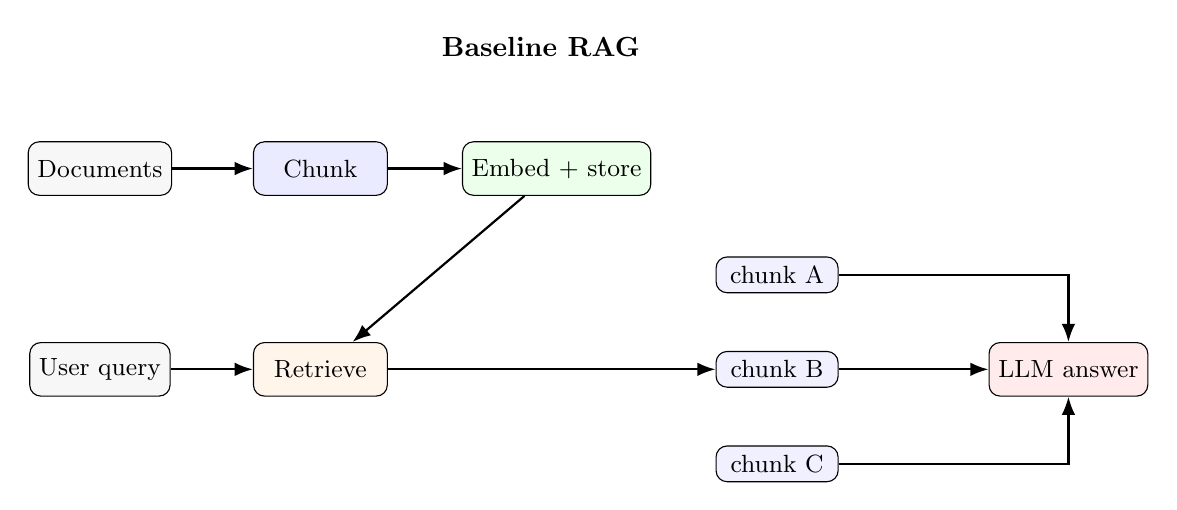
\begin{tikzpicture}[>=Latex, every node/.style={font=\small}]
    \tikzstyle{stage}=[draw, rounded corners, minimum width=1.7cm, minimum height=0.68cm, align=center]
    \tikzstyle{data}=[draw, rounded corners, minimum width=1.7cm, minimum height=0.68cm, align=center, fill=gray!6]
    \tikzstyle{chunkrow}=[draw, rounded corners, minimum width=1.55cm, minimum height=0.34cm, align=center, fill=blue!6]

    \node[font=\normalsize] at (6.8,3.1) {\textbf{Baseline RAG}};

    \node[data] (docsA) at (1.2,1.55) {Documents};
    \node[stage, fill=blue!8] (chunkA) at (4.0,1.55) {Chunk};
    \node[stage, fill=green!8] (embedA) at (7.0,1.55) {Embed + store};
    \draw[->, thick] (docsA) -- (chunkA);
    \draw[->, thick] (chunkA) -- (embedA);

    \node[data] (queryA) at (1.2,-1.0) {User query};
    \node[stage, fill=orange!8] (retrieveA) at (4.0,-1.0) {Retrieve};
    \draw[->, thick] (queryA) -- (retrieveA);
    \draw[->, thick] (embedA) -- (retrieveA);

    \node[chunkrow] (a1) at (9.8,0.2) {chunk A};
    \node[chunkrow] (a2) at (9.8,-1.0) {chunk B};
    \node[chunkrow] (a3) at (9.8,-2.2) {chunk C};
    \draw[->, thick] (retrieveA.east) -- (a2.west);

    \node[stage, fill=red!8] (genA) at (13.5,-1.0) {LLM answer};
    \draw[->, thick] (a1.east) -| (genA.north);
    \draw[->, thick] (a2.east) -- (genA.west);
    \draw[->, thick] (a3.east) -| (genA.south);
\end{tikzpicture}
}
\caption{Baseline RAG retrieves evidence and generates directly from it.}
\end{figure}

Many systems stop here. This is the standard architecture the reader
should understand by this point in the document: take documents, chunk
them, embed them, store them, retrieve relevant evidence, and generate an
answer from that evidence.

Some systems go one step further and add reranking after retrieval. A
reranker can often improve the final evidence set by reordering or
filtering the retrieved candidates more carefully. But at the time of
writing, reranking is still better understood as a more advanced RAG
pattern than as part of the default baseline. Many traditional systems
and many simpler production systems do not use a reranker at all.
This version can be stronger when the first-pass retriever finds the
right material but orders it imperfectly. Even so, it is optional. You do
not need reranking to understand or build a basic RAG system, and many
working systems still stop after retrieval and generation.

\begin{figure}[h]
\centering
\resizebox{\textwidth}{!}{%
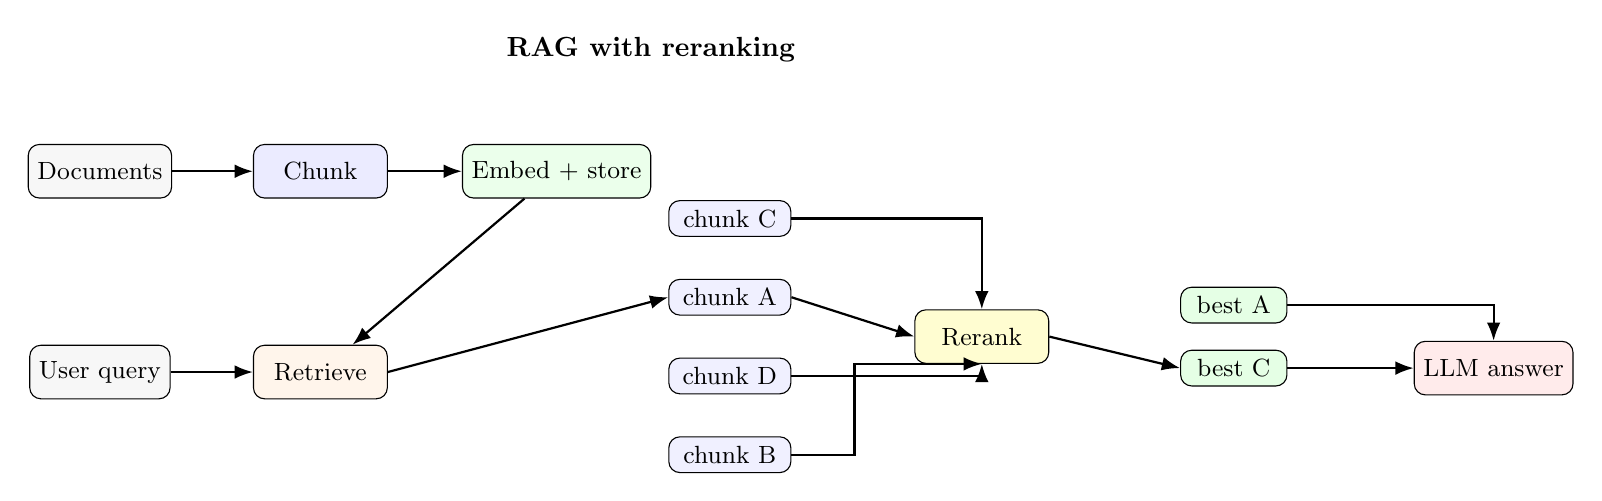
\begin{tikzpicture}[>=Latex, every node/.style={font=\small}]
    \tikzstyle{stage}=[draw, rounded corners, minimum width=1.7cm, minimum height=0.68cm, align=center]
    \tikzstyle{data}=[draw, rounded corners, minimum width=1.7cm, minimum height=0.68cm, align=center, fill=gray!6]
    \tikzstyle{chunkrow}=[draw, rounded corners, minimum width=1.55cm, minimum height=0.34cm, align=center, fill=blue!6]
    \tikzstyle{bestrow}=[draw, rounded corners, minimum width=1.35cm, minimum height=0.34cm, align=center, fill=green!10]

    \node[font=\normalsize] at (8.2,3.1) {\textbf{RAG with reranking}};

    \node[data] (docsB) at (1.2,1.55) {Documents};
    \node[stage, fill=blue!8] (chunkB) at (4.0,1.55) {Chunk};
    \node[stage, fill=green!8] (embedB) at (7.0,1.55) {Embed + store};
    \draw[->, thick] (docsB) -- (chunkB);
    \draw[->, thick] (chunkB) -- (embedB);

    \node[data] (queryB) at (1.2,-1.0) {User query};
    \node[stage, fill=orange!8] (retrieveB) at (4.0,-1.0) {Retrieve};
    \draw[->, thick] (queryB) -- (retrieveB);
    \draw[->, thick] (embedB) -- (retrieveB);

    \node[chunkrow] (c1) at (9.2,0.95) {chunk C};
    \node[chunkrow] (c2) at (9.2,-0.05) {chunk A};
    \node[chunkrow] (c3) at (9.2,-1.05) {chunk D};
    \node[chunkrow] (c4) at (9.2,-2.05) {chunk B};
    \draw[->, thick] (retrieveB.east) -- (c2.west);

    \node[stage, fill=yellow!18] (rerankB) at (12.4,-0.55) {Rerank};
    \draw[->, thick] (c1.east) -| (rerankB.north);
    \draw[->, thick] (c2.east) -- (rerankB.west);
    \draw[->, thick] (c3.east) -| (rerankB.south);
    \draw[->, thick] (c4.east) -- ++(0.8,0) |- (rerankB.south);

    \node[bestrow] (best1) at (15.6,-0.15) {best A};
    \node[bestrow] (best2) at (15.6,-0.95) {best C};
    \draw[->, thick] (rerankB.east) -- (best2.west);

    \node[stage, fill=red!8] (genB) at (18.9,-0.95) {LLM answer};
    \draw[->, thick] (best1.east) -| (genB.north);
    \draw[->, thick] (best2.east) -- (genB.west);
\end{tikzpicture}
}
\caption{Reranked RAG inserts an extra post-retrieval step that reorders or
filters candidate chunks before generation.}
\end{figure}

So the main thing to understand is that RAG is not one magical model. It
is a pipeline made from several design choices working together:
vectorization, storage, indexing, retrieval, and then generation from the
retrieved evidence. Reranking, fusion, and additional retrieval passes
can make that pipeline stronger, but they are later refinements on top of
the core architecture rather than the definition of RAG itself.

That basic pipeline is enough to explain a large fraction of practical
RAG systems. The rest of the document moves into more advanced concerns:
how to compress vectors, how to evaluate retrieval quality, how to plan
queries more intelligently, how agentic systems extend retrieval, and how
graph structure can complement vector search.

\section{Advanced Topics}

Prefacing this section by saying it's not comprehensive whatsoever and will honestly feel more like a collection of scattered thoughts than it will feel like a coherent, well structured explanation of improvements you can make to your RAG system. The reason I label these advanced however is not because they're meaningfully complicated, rather they are mostly unnecessary in most use cases.

As you'll read later, quantization isn't really meaningfully relevant to you unless your corpus starts nearing tens of millions of vectors. Evaluations are obviously very ideal in practice but often require a ton of labeling (and hence resources) that most entities aren't going to conduct. Agentic RAG and Knowledge graphs are amazing in theory but I've personally yet to convince myself of the fact that the additional expense is worth the potentially slight edge it may have over a properly made RAG system. 

\subsection{Quantization}

Vectors are expensive to store at scale. Suppose an embedding has 1536
dimensions and each coordinate is stored as a 32-bit float. Since a
32-bit float uses 4 bytes, one vector takes
\[
1536 \times 4 = 6144 \text{ bytes.}
\]
If we store $N$ such vectors, the raw storage for the vectors alone is
\[
N \times 6144 \text{ bytes.}
\]
That scales faster than it may feel at first glance. For 10,000 vectors,
the storage is $10{,}000 \times 6144 = 61{,}440{,}000$ bytes, or roughly
61 MB. For 1,000,000 vectors, it becomes $6{,}144{,}000{,}000$ bytes, or
roughly 6.1 GB. For 100,000,000 vectors, it becomes
$614{,}400{,}000{,}000$ bytes, or roughly 614 GB. And that is before any
metadata, indexing structures, replication, or operational overhead.

We can always try to store vectors in a distributed way by sharding them
across machines. That helps operationally, but it does not remove the
underlying storage cost. The total number of bytes still has to exist
somewhere. This is why compression matters: any meaningful reduction in
per-vector size can materially reduce the size of the vector store, along
with the memory pressure, hardware cost, and data movement that come with
it.

Quantization is one way to reduce that cost. The idea is to store vectors
with less precision than full 32-bit floating point values. Instead of
keeping every coordinate as a full float, we store a compressed
representation that is cheaper to keep in memory, cheaper to move through
the CPU or GPU, and sometimes faster to search.

The tradeoff is distortion. Once we compress a vector, it is no longer
exactly the same point in space. If the distortion is small, nearest
neighbors mostly stay the same. If the distortion is large, the system may
retrieve the wrong candidates.

\subsubsection{Scalar Quantization}

One natural idea is to ask: instead of storing each coordinate as a
32-bit float, why not store a smaller integer? For example, we might map
the original floating-point values into something like 8-bit integers.
That immediately cuts the storage needed for each coordinate and can also
reduce memory traffic during retrieval. The cost is that the vector is no
longer represented exactly. We have forced a continuous value into a much
smaller set of possible levels, so some geometric distortion is
unavoidable.

\subsubsection{Binary Quantization}

We can push the idea even further. Instead of storing smaller integers,
what if we store only binary information, such as signs or bit patterns?
That is a much more aggressive form of compression. At first that can
sound too lossy to be useful, but high-dimensional vectors often contain
enough aggregate variation that even extremely compressed
representations can still preserve useful retrieval signal. The tradeoff,
of course, is that binary quantization is giving up much more information
than scalar quantization, so the risk of hurting retrieval quality is
higher.

These are not the only quantization ideas, but they are a good place to
start because the logic behind them follows directly from the storage
problem itself.

The goal is not just smaller files. In retrieval, compression changes
speed, memory use, cache behavior, and sometimes recall. A quantized index
can be a huge win, but only if the search quality stays good enough for
the application.

\subsubsection{Quantization In Practice}

Quantization starts to make sense when storage or memory bandwidth is
actually hurting you. That usually means large vector collections, high
query volume, expensive RAM, or systems that need to keep a large share
of the index in memory. If the dataset is small, the latency budget is
loose, or retrieval quality is already shaky, quantization may solve the
wrong problem.

The only way to judge it is to test it. Take the compressed system and
compare it against a full-precision baseline on the same queries. Measure
\texttt{recall@k}, nDCG or MRR if you have labels, along with latency,
index size, build time, memory use, and end-to-end answer quality. If the
retriever feeds a language model, that last metric matters more than it
first appears to. The real question is not just whether the nearest
neighbors moved around a little. It is whether the model still gets the
right evidence and produces the right answer.

TurboQuant is one example of recent work here. The
\href{https://arxiv.org/abs/2504.19874}{TurboQuant paper} describes an
online vector quantization method meant to preserve geometric structure
while cutting memory use. The paper reports low distortion,
inner-product preservation through a residual correction step, strong
results for KV-cache compression, and better nearest-neighbor search
results than the product quantization baselines it compares against.

Those are research results, not a reason to compress everything by
default. Whether a method like TurboQuant helps depends on the embedding
model, the dataset, the hardware, the index, and how much missed
retrieval the application can tolerate. In practice, the test is simple:
compress the vectors, run the same benchmark, and see what changed. If
storage and latency improve without pushing recall or answer quality below
the level you need, the compression is probably worth it. If the system
starts missing evidence that mattered before, it probably is not.

\subsection{Evaluation}

Evaluation is where retrieval systems stop being plausible and start being
credible. Once a RAG pipeline is in place, the next question is whether
it actually retrieves the right evidence and whether the final generated
answer is grounded in that evidence. This area is active and still moving
quickly, but a few evaluation patterns show up repeatedly in both
practical systems and recent literature.

\subsubsection{Offline retrieval evaluation}

The basic setup is simple. Start with a query set. For each query, decide
which chunks count as relevant evidence. Then run the retriever and look
at the ranked list it returns. That gives you the core object retrieval
evaluation works with: a query, a ground-truth notion of relevance, and
an ordered result list.

The reason ranking matters is that retrieval is not only about whether a
useful chunk appears somewhere. It is also about where it appears. In a
RAG system, the top of the list gets the most attention. If the relevant
evidence is buried too far down, the language model may never see it, or
it may receive it too late and with too much noise around it.

Take a small example. Suppose the query is:
\begin{quote}
``What changed in the 2024 return policy?''
\end{quote}
and the retriever returns these top four chunks:
\begin{enumerate}
    \item chunk A: a shipping FAQ
    \item chunk B: the 2024 return policy update
    \item chunk C: a warranty page
    \item chunk D: a summary of return exceptions
\end{enumerate}
Assume chunks B and D are the relevant evidence for this query.

\paragraph{\texttt{recall@k}}

One natural question is: did the retriever surface the relevant evidence
within the first $k$ results? That is the idea behind
\texttt{recall@k}. In this example, \texttt{recall@1} is 0 because the
first result is not relevant. \texttt{recall@2} is $1/2$ because one of
the two relevant chunks has appeared in the top two. \texttt{recall@4} is
$2/2 = 1$ because both relevant chunks appear within the top four.
This metric is useful when coverage matters more than fine ordering. That
often happens in RAG, where missing a key chunk can hurt more than having
the right chunk in position 2 instead of position 1.

\paragraph{MRR}

Another question is: how far down the ranking do we have to go before we
hit the first relevant result? In the example above, the first relevant
chunk appears at rank 2. The reciprocal of that rank is $1/2$. That is
the per-query reciprocal rank. Mean reciprocal rank, or MRR, is just the
average of that quantity across many queries. MRR is useful when you care
strongly about getting at least one good hit very early. Its limitation is
that it pays attention only to the first relevant result. If the task
needs several relevant chunks, MRR can look healthy even when the rest of
the evidence is ordered poorly.

\paragraph{nDCG}

Some tasks need a finer notion of relevance than yes or no. Maybe one
chunk contains the exact policy change, another contains a partial
summary, and another only provides weak supporting context. That is where
nDCG becomes useful. The logic is straightforward: more relevant items
should appear earlier, lower positions should count less, and the score
should be normalized against the best possible ranking.

Using the same top four results, suppose the graded relevance labels are:
chunk A = 1, chunk B = 3, chunk C = 0, and chunk D = 2. Then the
retriever's ranking has gains $[1,3,0,2]$. A common discounted cumulative
gain is
\[
\mathrm{DCG}@4 =
\frac{2^1-1}{\log_2(1+1)} +
\frac{2^3-1}{\log_2(2+1)} +
\frac{2^0-1}{\log_2(3+1)} +
\frac{2^2-1}{\log_2(4+1)}.
\]
Numerically, that is about
\[
1 + \frac{7}{\log_2 3} + 0 + \frac{3}{\log_2 5} \approx 6.71.
\]
If we sort the same gains into the ideal ranking $[3,2,1,0]$, then
\[
\mathrm{IDCG}@4 =
7 + \frac{3}{\log_2 3} + \frac{1}{\log_2 4} + 0 \approx 9.39.
\]
So
\[
\mathrm{nDCG}@4 = \frac{\mathrm{DCG}@4}{\mathrm{IDCG}@4}
\approx \frac{6.71}{9.39} \approx 0.71.
\]
The exact number matters less than the interpretation: the ranking is not
terrible, but it is clearly worse than the ideal ordering because the
best evidence is not at the top.

\paragraph{Comparing the metrics}

In practice, these metrics answer different questions. \texttt{recall@k}
is good for evidence coverage. MRR is good for early first-hit quality.
nDCG is good for ranking quality when relevance is graded. Teams often
track more than one of them because each exposes a different failure mode.
This is also why offline retrieval evaluation is useful: it isolates the
retriever and makes it easier to compare chunking strategies, embedding
models, indexes, and rerankers before generation enters the picture.

\subsubsection{End-to-end answer evaluation}

Another approach is to evaluate the whole RAG system at the answer level.
Here the question is not only whether the right chunk was retrieved, but
whether the final answer is correct, supported, and complete enough for
the task. A system can retrieve the right chunk and still give a weak
answer because the prompt is poor, the model overgeneralizes, or the
evidence is not used well. The reverse can also happen: the retriever can
be imperfect, but the final answer is still good enough for the user.

That is why answer-level evaluation usually asks several separate
questions. Is the answer factually correct? Is it grounded in retrieved
evidence rather than invented? Does it include the important parts of the
answer, or is it incomplete? And for the actual use case, is it useful
enough to help the user finish the task they came to do?

\subsubsection{Synthetic data and judge-based evaluation}

Recent systems often use synthetic queries, synthetic labels, or
LLM-as-judge workflows to scale evaluation when human labels are
expensive. The appeal is obvious: hand-labeling retrieval data is slow and
costly, and answer-level review is even more expensive. Synthetic queries
can expand a test set quickly, and LLM judges can score answers at a much
lower cost than full human review.

The catch is that these methods can fail in recognizable ways. Synthetic
queries may not look like real user behavior. Synthetic labels may reflect
the assumptions of the generator rather than the real task. A model that
judges another model can drift toward self-confirming behavior, especially
if both share similar weaknesses. And even a strong judge can be
inconsistent across domains or prompt formulations.

So these methods are useful, but they are best treated as scaling tools
for iteration rather than as unquestioned ground truth. In practice, they
work best when they are calibrated against at least some human judgments.

\subsection{Query Planning}

Basic retrieval takes a query and runs it once. More advanced systems try
to decide how the query should be handled before retrieval happens. That
planning layer is increasingly important in modern RAG because many real
questions are ambiguous, multi-hop, or better answered by a sequence of
retrieval steps rather than a single search.

\subsubsection{Query rewriting and decomposition}

Embedding the raw user query is not always the best move. The question in
your head and the query you would actually type into Google are often not
the same thing. Human questions are frequently conversational, indirect,
or missing the exact words that matter for retrieval. A retriever often
benefits from a cleaner, more explicit version of the same intent.

For example, imagine a user asks:
\begin{quote}
``I'm trying to remember the rule about when you can still return
something even if it's already been opened.''
\end{quote}
That is a perfectly natural question, but it is not an ideal retrieval
query. A rewritten version might be:
\begin{quote}
``opened product return policy exceptions''
\end{quote}
The rewritten query adds the key terms ``return policy'' and
``exceptions,'' removes filler, and makes the retrieval target much more
obvious.

Here is a different failure mode. Suppose the user asks:
\begin{quote}
``Why does that electric SUV lose range so badly in the winter?''
\end{quote}
If the document collection is full of technical product information, the
retriever may do better with something like:
\begin{quote}
``electric SUV winter range loss battery temperature efficiency''
\end{quote}
This rewrite adds missing retrieval terms that the user implied but did
not say directly. The user asked a natural question. The retriever often
wants something closer to a search query.

Sometimes rewriting is still not enough because the question actually
contains several retrieval problems at once. For example:
\begin{quote}
``Which database should we use for support-ticket search, and how would
we evaluate whether it is better than our current setup?''
\end{quote}
That can be decomposed into at least two sub-queries: one about database
options for retrieval, and another about evaluation methodology. In cases
like that, decomposition helps because the system is no longer forcing one
retrieval pass to answer two different questions.

\subsubsection{Routing and retriever selection}

Once the system has a cleaner version of the query, it may also choose a
better retrieval route. Not every query should go through the same
pipeline. Some queries want exact lexical matching. Others benefit from
semantic search or a hybrid approach.

For instance, a query like
\begin{quote}
``Toyota RAV4 2021 towing capacity AWD''
\end{quote}
is heavily keyword-driven. Exact model names, years, and trims matter, so
a lexical or BM25-heavy route is a natural choice. But a query like
\begin{quote}
``family car good for snow and road trips''
\end{quote}
is much fuzzier. That kind of query often benefits from semantic search
or a hybrid retriever that combines lexical and embedding-based signals.
Planning is not only about rewriting the query. It is also about choosing
where that query should go.

\subsubsection{Multi-step retrieval plans}

Some questions should not be answered in one retrieval pass at all. A
stronger pattern is to retrieve, inspect what came back, and then decide
what to retrieve next.

For example, suppose a user asks:
\begin{quote}
``Why did last quarter's returns spike?''
\end{quote}
The first retrieval pass might surface documents showing that most returns
came from one product line. At that point the next retrieval step becomes
clearer: search specifically for defects, shipping issues, or policy
changes related to that product line. The second query is better because
the first retrieval step told us what the real issue probably is.

This is why query planning matters. Retrieval is not always one clean
lookup against a perfectly phrased query. Sometimes the system needs to
rewrite the question, sometimes it needs to split it apart, and sometimes
it needs one retrieval step to figure out what the next retrieval step
should be.

\subsection{Agentic RAG}

Query planning already introduced several ways to improve retrieval before
the main search happens: rewriting the query, routing it to a better
retriever, or decomposing the task into several steps. Agentic RAG is the
next move beyond that. The difference is not just that the system takes
more steps. The difference is that it can react to the evidence that comes
back while retrieval is in progress.

That distinction matters. Query planning decides how to search before the
results are known. Agentic RAG can revise that decision after seeing what
retrieval actually produced. In that sense, retrieval becomes a feedback
process rather than a one-shot lookup.

\subsubsection{Tool use and iterative retrieval}

The first retrieval pass often does not answer the question directly. It
may only reveal the shape of the problem. That is still useful because the
system can use the first batch of evidence to decide what to retrieve next.

Suppose a user asks:
\begin{quote}
``Why did payment failures spike last night?''
\end{quote}
That is too vague for one perfect retrieval step. A first pass over
incident notes, dashboards, and alerts might surface repeated references
to one payment gateway or one error family such as ``3DS challenge
timeouts.'' Once that focal entity appears, the second retrieval step
becomes much sharper: search specifically for that gateway, that timeout
class, recent deploys touching that path, and similar incidents. The first
search did not solve the problem. It exposed where the evidence probably
lives.

This is the practical meaning of iterative retrieval. The system is not
performing extra tool use for its own sake. It is gathering evidence in
stages, where each retrieval pass makes the next one more targeted.

\subsubsection{Reflection and self-correction}

Reflection and self-correction are the stronger version of this pattern.
The system retrieves evidence, inspects whether it is relevant,
contradictory, or noisy, and then decides how to correct retrieval before
it answers. The important move is not ``think harder.'' The important move
is ``use the returned evidence to improve the next search.''

One useful mechanism is positive and negative retrieval guidance. A
positive example is a retrieved chunk that looks like the kind of evidence
the system wants more of. A negative example is a chunk that is loosely
related in embedding space but is actually distracting, off-target, or
from the wrong subdomain. This matters especially for vector search, where
semantic similarity can pull in material that is nearby in meaning but not
nearby in operational usefulness. If the retriever can take both ``more
like this'' and ``less like this'' signals, the next search can move
toward a better evidence neighborhood.

Consider an ambiguous support question:
\begin{quote}
``Can I still send it back if I opened the box?''
\end{quote}
An initial vector search might return a mix of return-policy chunks and
warranty pages because both talk about eligibility, product condition, and
customer remedies. After seeing those results, the system can mark one
return-policy chunk as a positive example and one warranty chunk as a
negative example, then run retrieval again with that guidance. The
improvement here is not just query rewriting. Rewriting changes the query
before retrieval. Reflection changes retrieval after the system has seen
that the current evidence is mixing two different policy neighborhoods.

Now consider a product or incident analysis question:
\begin{quote}
``What explains the recent failures in this device line?''
\end{quote}
The first pass might retrieve documents about several superficially
similar product lines, along with multiple possible causes. Suppose one
defect report clearly matches the failure symptoms while a shipping-delay
report appears only because it mentions the same product family and time
window. The system can treat the defect report as a positive example and
the shipping-delay report as a negative example, then issue another vector
search guided by both signals. That second pass moves toward the right
cluster of evidence. Again, this is different from plain query rewriting.
The correction depends on what retrieval produced, not just on a cleaner
phrasing of the original question.

The reason this works is simple. The first retrieval pass is often useful
even when it is imperfect. Partial or bad results still reveal what the
system should avoid and what it should chase. That turns retrieval into a
feedback loop: the initial pass generates evidence, the system judges that
evidence, and the next pass is shaped by that judgment.

\subsubsection{Long-horizon workflows}

At the broadest end of the design space, retrieval sits inside a longer
memory, planning, and action loop that can run over many turns. Those
systems may be useful for larger tasks, but they are also much harder to
control and evaluate, so the core retrieval story here is still the
shorter feedback loop of retrieve, inspect, and retrieve again.

\end{document}
